\documentclass[11pt,a4paper]{article}
\usepackage[a4paper,top=1.8cm,bottom=1.9cm,left=1.9cm,right=1.9cm]{geometry}
\usepackage{fontspec}
\setmainfont{Noto Serif}
\setsansfont{Noto Sans}
\usepackage{microtype}
\usepackage{xcolor}
\usepackage{hyperref}
\usepackage{booktabs,tabularx,array,multicol}
\usepackage{enumitem}
\usepackage{tikz}
\usetikzlibrary{positioning,arrows.meta,shapes.geometric,fit}
\usepackage[most]{tcolorbox}
\usepackage{fancyhdr,lastpage}
\usepackage{xurl}
\usepackage{float}
\usepackage{caption}
\usepackage{amssymb}
\usepackage{pgfplots}
\pgfplotsset{compat=1.18}

\definecolor{Navy}{HTML}{0F172A}
\definecolor{Slate}{HTML}{334155}
\definecolor{Muted}{HTML}{64748B}
\definecolor{Green}{HTML}{059669}
\definecolor{Mint}{HTML}{D1FAE5}
\definecolor{Light}{HTML}{F8FAFC}
\definecolor{Border}{HTML}{CBD5E1}
\definecolor{Amber}{HTML}{B45309}
\definecolor{Blue}{HTML}{2563EB}

\hypersetup{colorlinks=true,linkcolor=Navy,urlcolor=Blue,citecolor=Green,pdftitle={PineGuard Final Project Report},pdfauthor={Chung-Yu Cheng}}
\pagestyle{fancy}
\fancyhf{}
\lhead{\sffamily\small PineGuard}
\rhead{\sffamily\small r12323059}
\cfoot{\sffamily\small \thepage\,/\,\pageref{LastPage}}
\renewcommand{\headrulewidth}{0.25pt}
\setlength{\parskip}{0.42em}
\setlength{\parindent}{0pt}
\setlength{\emergencystretch}{2em}

\usepackage{titlesec}
\titleformat{\section}{\Large\sffamily\bfseries\color{Navy}}{\thesection}{0.65em}{}
\titleformat{\subsection}{\large\sffamily\bfseries\color{Slate}}{\thesubsection}{0.55em}{}
\titlespacing*{\section}{0pt}{1.0em}{0.36em}
\titlespacing*{\subsection}{0pt}{0.7em}{0.18em}

\newtcolorbox{keybox}[1]{enhanced,colback=Light,colframe=Border,coltitle=Navy,title={\sffamily\bfseries #1},boxrule=0.5pt,arc=3mm,left=3mm,right=3mm,top=2mm,bottom=2mm}
\newtcolorbox{claimbox}{enhanced,colback=Navy,colframe=Navy,coltext=white,boxrule=0pt,arc=4mm,left=4mm,right=4mm,top=3mm,bottom=3mm}
\newcommand{\src}[1]{\textsuperscript{[#1]}}
\newcommand{\RepoURL}{\href{https://github.com/r12922076/bda\_final}{https://github.com/r12922076/bda\_final}}
\newcommand{\LiveURL}{\href{https://r12922076.github.io/bda\_final/}{https://r12922076.github.io/bda\_final/}}

\begin{document}

\begin{titlepage}
\thispagestyle{empty}
\begin{tikzpicture}[remember picture,overlay]
  \fill[Light] (current page.south west) rectangle (current page.north east);
  \fill[Navy] (current page.north west) rectangle ([yshift=-12.9cm]current page.north east);
  \fill[Green] ([xshift=-3.15cm,yshift=-2.25cm]current page.north east) circle (2.25cm);
  \fill[Mint,opacity=.15] ([xshift=-4.05cm,yshift=-6.85cm]current page.north east) circle (2.80cm);
  \draw[Green,line width=1.2pt] ([xshift=1.9cm,yshift=-12.9cm]current page.north west) -- ([xshift=-1.9cm,yshift=-12.9cm]current page.north east);
\end{tikzpicture}
\vspace*{0.45cm}
{\sffamily\bfseries\color{Mint}\large Big Data Systems Final Project}\par
\vspace{0.85cm}
{\sffamily\bfseries\color{white}\fontsize{34}{38}\selectfont PineGuard}\par
\vspace{0.25cm}
{\sffamily\bfseries\color{white}\fontsize{16.5}{21}\selectfont TradingView Strategy Workflow Trust Layer}\par
\vspace{0.12cm}
{\sffamily\color{Mint}\fontsize{12.5}{17}\selectfont Monetizing auditable strategy workflow validation, not trading alpha}\par
\vspace{0.55cm}
{\sffamily\small\color{white}%
\fcolorbox{Mint}{Navy}{\strut\hspace{0.45em}Data product\hspace{0.45em}}\hspace{0.45em}%
\fcolorbox{Mint}{Navy}{\strut\hspace{0.45em}Static deployed prototype\hspace{0.45em}}\hspace{0.45em}%
\fcolorbox{Mint}{Navy}{\strut\hspace{0.45em}Evidence-backed report\hspace{0.45em}}% 
}\par
\vspace{0.62cm}
\begin{tcolorbox}[enhanced,width=.90\textwidth,colback=white,colframe=white,boxrule=0pt,arc=3mm,left=3.5mm,right=3.5mm,top=2.8mm,bottom=2.8mm]
\sffamily\small\color{Navy}
\begin{tabularx}{\linewidth}{@{}>{\bfseries\color{Slate}}p{4.2cm}X@{}}
Student ID & \textcolor{Green}{\textbf{r12323059}} \\
GitHub Repository & \RepoURL \\
Live Demo & \LiveURL \\
\end{tabularx}
\end{tcolorbox}

\vspace{2.55cm}
\noindent
\begin{minipage}[t]{0.31\textwidth}
\begin{tcolorbox}[enhanced,colback=white,colframe=Border,boxrule=0.45pt,arc=3mm,left=2.5mm,right=2.5mm,top=2mm,bottom=2mm,height=3.15cm]
{\sffamily\bfseries\color{Green}Initial wedge}\par\vspace{0.12cm}
{\sffamily\small \raggedright\hyphenpenalty=10000\exhyphenpenalty=10000 Paid users with alert logs ready for review.}
\end{tcolorbox}
\end{minipage}\hfill
\begin{minipage}[t]{0.31\textwidth}
\begin{tcolorbox}[enhanced,colback=white,colframe=Border,boxrule=0.45pt,arc=3mm,left=2.5mm,right=2.5mm,top=2mm,bottom=2mm,height=3.15cm]
{\sffamily\bfseries\color{Green}Monetized data}\par\vspace{0.12cm}
{\sffamily\small \raggedright\hyphenpenalty=10000\exhyphenpenalty=10000 Alerts, metadata, evidence labels, rules, and report log.}
\end{tcolorbox}
\end{minipage}\hfill
\begin{minipage}[t]{0.31\textwidth}
\begin{tcolorbox}[enhanced,colback=white,colframe=Border,boxrule=0.45pt,arc=3mm,left=2.5mm,right=2.5mm,top=2mm,bottom=2mm,height=3.15cm]
{\sffamily\bfseries\color{Green}Delivered product}\par\vspace{0.12cm}
{\sffamily\small \raggedright\hyphenpenalty=10000\exhyphenpenalty=10000 Report, monitor, explorer, and tour.}
\end{tcolorbox}
\end{minipage}

\vfill
\begin{claimbox}
\sffamily\textbf{Core thesis.} PineGuard does not sell trading signals, promise returns, or execute trades. It converts fragmented TradingView-style workflow data into an auditable paid health report and monitoring dashboard.
\end{claimbox}
\vspace{0.55cm}
{\sffamily\small\color{Slate}National Taiwan University \hfill June 2026}\par
\end{titlepage}

\tableofcontents
\newpage

\section{Executive Summary}

PineGuard is a static, deployed data-product prototype for paid or power TradingView users who already use alerts, Pine Script indicators, Strategy Tester, webhooks, or paid scripts, but lack a structured validation workflow. The beachhead customer is the alert-heavy paid TradingView user: this user already generates alert-event data, already invests in trading workflow tools, and already faces the operational problem of knowing whether a strategy is credible after it leaves the chart.

\begin{keybox}{Product boundary}
PineGuard is workflow validation, not investment advice. Its output is a strategy health report: score breakdown, missing workflow components, forward-test outcome summary, evidence basis, and recommended next validation step. The score measures workflow completeness and evidence quality; it does not estimate expected profitability.
\end{keybox}

The deployed artifact is a static single-page application on GitHub Pages. It contains routes for a landing page, health-check wizard, diagnosis page, strategy-template library, forward-test monitor, evidence explorer, downloadable report, pricing page, architecture page, risk page, and documentation hub. The production architecture is specified separately as an event-driven system with webhook ingestion, durable queues, validation workers, relational metadata storage, raw payload storage, scheduled recomputation, and report delivery.

\section{Target Customer and Wedge}

The initial customer is an individual power user or small trading team that uses TradingView as the front end for discretionary or semi-systematic decision support. The first wedge is narrower than the full TradingView user base:

\begin{table}[H]
\centering
\caption{Beachhead and expansion segments}
\begin{tabularx}{\textwidth}{>{\raggedright\arraybackslash}p{3.1cm}X>{\raggedright\arraybackslash}p{3.2cm}}
\toprule
\textbf{Segment} & \textbf{Current workaround} & \textbf{PineGuard product} \\
\midrule
Alert-heavy paid TradingView user & Configures many alerts, then manually checks charts, screenshots, spreadsheets, or memory to judge outcomes. & Strategy Health Check and Forward-Test Monitor. \\
Pine Script builder & Uses Strategy Tester and code inspection but may miss repainting, lookahead, or unrealistic execution assumptions. & Health Check and Pro Completion Plan. \\
Paid-script buyer & Evaluates public claims or invite-only scripts with limited source-code visibility. & Later expansion: due-diligence checklist. \\
Indicator creator & Wants credibility artifacts without promising returns. & Later expansion: Creator Trust Report. \\
\bottomrule
\end{tabularx}
\end{table}

The product starts with alert-heavy users because they already produce the event data PineGuard needs. This makes the first monetizable workflow concrete: import or forward alerts, evaluate future outcomes, diagnose missing workflow components, and generate a report. PineGuard therefore acts as a trust layer between TradingView strategy development and any later execution bridge or manual trading decision.

\section{Demand Evidence and Willingness to Pay}

The demand case uses public digital traces rather than private interviews. The evidence dataset contains official documentation, public script or marketplace traces, competitor or adjacent product pages, pricing references, and manually coded public evidence. The evidence is directional, not a representative survey. It is still useful because it distinguishes direct technical evidence from indirect willingness-to-pay benchmarks. The report treats public-evidence-derived personas as synthetic workflow summaries rather than interview respondents.

\subsection{Evidence acquisition process}

\begin{table}[H]
\centering
\caption{Evidence acquisition and coding workflow}
\small
\begin{tabularx}{\textwidth}{>{\raggedright\arraybackslash}p{3.0cm}X>{\raggedright\arraybackslash}p{3.1cm}}
\toprule
\textbf{Step} & \textbf{Procedure} & \textbf{Output} \\
\midrule
Seed selection & Start from TradingView official pages, alert/webhook documentation, Pine Script documentation, public scripts, competitor pages, and pricing pages. & Seed URL table. \\
Collection & Keep public pages only and avoid login-only, private, or paywalled content. & Raw public evidence rows. \\
Manual coding & Assign source type, pain category, relevance note, evidence role, and strength label. & Combined evidence snapshot. \\
Build step & Convert CSV evidence, alert events, strategy templates, and market snapshots into a single static JSON file. & Runtime data for GitHub Pages SPA. \\
Validation & Run static-site and frontend smoke tests. & Reproducibility checks. \\
\bottomrule
\end{tabularx}
\end{table}

Evidence strength is intentionally conservative. Official documentation is marked as strong technical evidence. Competitor pricing and adjacent-product pages are medium willingness-to-pay benchmarks. Marketplace listings are weaker demand proxies.

\subsection{Evidence governance and limitations}

The evidence supports a defensible beachhead hypothesis, not proven product-market fit. PineGuard's demand claim is deliberately conservative: paid TradingView users already generate strategy-workflow data, public sources document validation pain, and adjacent tools show that this audience pays for workflow infrastructure. A real launch would still require direct interviews, landing-page conversion tests, and retention metrics.

\begin{table}[H]
\centering
\caption{Evidence types and conservative interpretation}
\small
\begin{tabularx}{\textwidth}{>{\raggedright\arraybackslash}p{3.2cm}X>{\raggedright\arraybackslash}p{3.0cm}}
\toprule
\textbf{Evidence type} & \textbf{What it supports} & \textbf{Limitation} \\
\midrule
Official platform documents & Alerts, webhooks, repainting, Strategy Tester assumptions, and Pine Script behavior are real platform-level topics. & Technical validity, not willingness to pay. \\
Academic or professional validation sources & Backtest overfitting, lookahead, transaction costs, and slippage are recognized strategy-validation risks. & Not always specific to retail TradingView users. \\
Public user discussions & Qualitative pain around backtest/live gaps, alert tracking, paid-script opacity, and manual workarounds. & Self-selected and non-representative. \\
Competitor pricing & Adjacent trading workflow, journal, automation, and research tools are monetized. & Indirect WTP benchmark, not PineGuard's demand curve. \\
Marketplace listings & Non-repaint, webhook, and backtest language appears in public strategy claims. & Promotional and weaker as demand evidence. \\
\bottomrule
\end{tabularx}
\end{table}

\subsection{Evidence categories}

\begin{figure}[H]
\centering
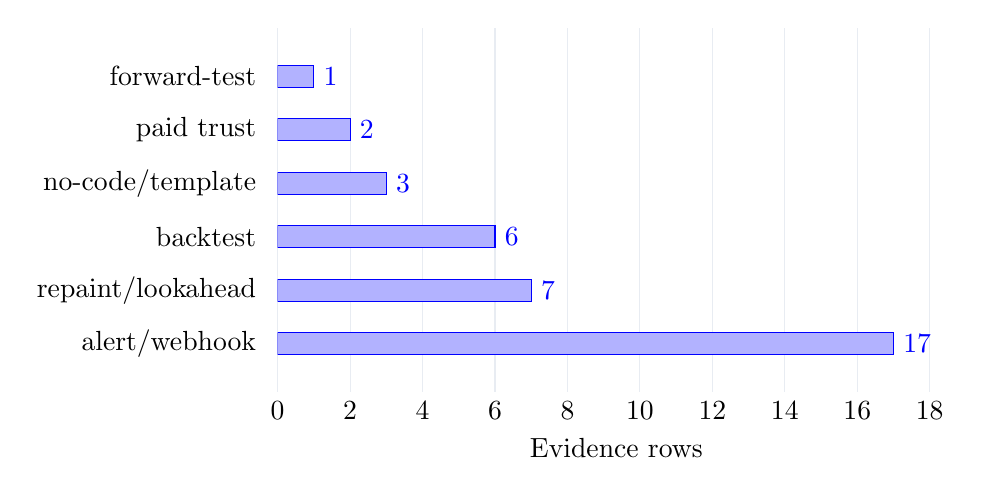
\begin{tikzpicture}
\begin{axis}[width=.84\textwidth,height=6.2cm,xbar,xmin=0,xlabel={Evidence rows},symbolic y coords={alert/webhook,repaint/lookahead,backtest,no-code/template,paid trust,forward-test},ytick=data,nodes near coords,bar width=8pt,enlarge y limits=.18,axis line style={draw=none},tick style={draw=none},xmajorgrids=true,grid style={draw=Border!45},every axis plot/.append style={fill=Green!75,draw=Green!75}]
\addplot coordinates {(17,alert/webhook) (7,repaint/lookahead) (6,backtest) (3,no-code/template) (2,paid trust) (1,forward-test)};
\end{axis}
\end{tikzpicture}
\caption{Evidence rows by pain category in the static evidence snapshot.}
\end{figure}

\begin{table}[H]
\centering
\caption{Evidence role by strength label in the current snapshot}
\small
\begin{tabularx}{\textwidth}{>{\raggedright\arraybackslash}p{4.2cm}>{\centering\arraybackslash}p{1.8cm}>{\centering\arraybackslash}p{1.8cm}>{\centering\arraybackslash}p{1.8cm}X}
\toprule
\textbf{Evidence role} & \textbf{Strong} & \textbf{Medium} & \textbf{Weak} & \textbf{Interpretation} \\
\midrule
Technical validity evidence & 14 & 0 & 0 & Platform mechanics and validation failure modes are directly documented. \\
Adjacent-market benchmark & 0 & 13 & 0 & Pricing and product benchmarks support adjacent willingness-to-pay, not direct demand. \\
Demand proxy & 0 & 3 & 5 & Public pain signals are directional and non-representative. \\
WTP benchmark evidence & 0 & 1 & 0 & One row directly supports pricing logic, but it is still not a conversion test. \\
\bottomrule
\end{tabularx}
\end{table}

The strongest technical evidence concerns repainting, backtest realism, and webhook/alert workflows. TradingView documentation discusses repainting as historical-versus-realtime behavior differences\src{1}, strategy testing assumptions such as order behavior, commission, and slippage\src{2}, and webhook alert delivery through HTTP POST requests\src{3}. These sources do not prove willingness to pay, but they establish that PineGuard addresses real workflow properties rather than invented concerns.

\subsection{Willingness to pay}

PineGuard's price corridor is benchmarked from adjacent products rather than a direct customer survey. This is an adjacent willingness-to-pay benchmark, not direct proof of PineGuard demand. Users already pay for TradingView, webhook automation, trading journals, and strategy-testing platforms. PineGuard should price below execution-routing tools because it validates rather than routes orders.

\begin{table}[H]
\centering
\caption{Adjacent-product benchmarks and PineGuard interpretation}
\scriptsize
\begin{tabularx}{\textwidth}{>{\raggedright\arraybackslash}p{2.55cm}>{\raggedright\arraybackslash}p{3.2cm}>{\raggedright\arraybackslash}p{3.25cm}X}
\toprule
\textbf{Category} & \textbf{Examples} & \textbf{Public benchmark source} & \textbf{Interpretation} \\
\midrule
Trading workflow platform & TradingView paid plans\src{4} & Paid plans tied to alerts, indicators, history, and workflow capacity. & The target segment already pays for trading tools. \\
Webhook automation & TradersPost; PickMyTrade; CrossTrade\src{11,12,13} & Public pricing and comparison pages show monthly alert-routing infrastructure products. & PineGuard should price below execution-routing tools because it validates rather than routes orders. \\
Trading journals and analytics & TradeZella; Edgewonk; TraderSync\src{14,15} & Trading journals monetize structured post-trade analytics and reports. & Supports one-time reports and monthly monitoring around strategy workflows. \\
Backtesting and research & TrendSpider; QuantConnect\src{16,17} & Research and backtesting platforms use premium subscriptions or paid platform access. & Supports paid strategy-evaluation products, but remains an adjacent benchmark. \\
\bottomrule
\end{tabularx}
\end{table}

The proposed entry pricing is USD 19-49 for a one-time Strategy Health Check and USD 19-39/month for a Forward-Test Monitor. In non-monetary terms, PineGuard replaces manual alert review, screenshots, spreadsheet tracking, and informal paid-script due diligence.

\section{Data Product and Business Model}

PineGuard monetizes the structured interpretation of strategy workflow data. Raw alerts and public URLs are not the product. The paid product is the validated report and monitoring workflow. In ecosystem terms, TradingView creates and displays strategies, execution bridges can route alerts to brokers, and PineGuard occupies the missing validation layer between those two steps.

\begin{table}[H]
\centering
\caption{Data-to-product mapping}
\begin{tabularx}{\textwidth}{>{\raggedright\arraybackslash}p{3.2cm}X>{\raggedright\arraybackslash}p{3.2cm}}
\toprule
\textbf{Input data} & \textbf{Processing} & \textbf{Output} \\
\midrule
Alert-event logs & Join alert timestamp, direction, symbol, and future price snapshot. & Forward-test outcome table. \\
Strategy metadata & Check missing cost assumptions, exits, versioning, repaint review, and payload schema. & Health score and gap diagnosis. \\
Public evidence rows & Label source type, pain category, evidence role, and evidence strength. & Evidence Explorer and report basis. \\
User profile & Match style, market, risk tolerance, and concerns to validation templates. & Recommended next validation modules. \\
\bottomrule
\end{tabularx}
\end{table}

\subsection{Health-score rationale}

The score is intentionally a workflow-completeness score. It makes no profitability claim. The weights are fixed and auditable so users can see why a report changes when a missing workflow component is added.

\begin{table}[H]
\centering
\caption{Health-score weights used in the browser-side scoring logic}
\small
\begin{tabularx}{\textwidth}{>{\raggedright\arraybackslash}p{3.4cm}>{\centering\arraybackslash}p{1.6cm}X}
\toprule
\textbf{Category} & \textbf{Max} & \textbf{Reason for weight} \\
\midrule
Backtest realism & 25 & Strategy Tester evidence is fragile when cost, slippage, and execution assumptions are missing. \\
Live alert observability & 20 & TradingView alerts become valuable data only when alert history and payload schema are captured. \\
Repainting/lookahead review & 20 & Multi-timeframe and realtime/historical differences are TradingView-specific failure modes. \\
Risk-rule completeness & 20 & A workflow is incomplete without exit logic and position-sizing assumptions. \\
Evidence quality & 15 & Forward-test records and version history make the report auditable. \\
\bottomrule
\end{tabularx}
\end{table}

\section{Technical Architecture}

\subsection{Deployed static SPA}

The deployed system is a static GitHub Pages application. It uses pre-built CSV/JSON snapshots and browser-side JavaScript. This is appropriate for the course artifact because the goal is to demonstrate the data product without requiring private backend credentials. The current prototype does not receive live webhooks, store private strategy data, or use DuckDB-Wasm at runtime; local OLAP processing is a production extension, not a claim about the demo.

\begin{table}[H]
\centering
\caption{Deployed SPA routes}
\small
\begin{tabularx}{\textwidth}{>{\raggedright\arraybackslash}p{3.1cm}X}
\toprule
\textbf{Route} & \textbf{Purpose} \\
\midrule
\texttt{\#/tour} & Two-minute grader path through the deployed artifact. \\
\texttt{\#/health-check} & Five-step wizard for persona, strategy profile, available data, and risk concerns. \\
\texttt{\#/diagnosis} & Health score, category breakdown, and missing workflow components. \\
\texttt{\#/monitor} & Forward-test monitor with horizon controls, sample CSV download, and webhook payload copy. \\
\texttt{\#/evidence} & Filterable evidence explorer with source type, pain category, and evidence strength. \\
\texttt{\#/report} & Downloadable Markdown/JSON Strategy Health Report. \\
\texttt{\#/architecture} & Static and production architecture. \\
\bottomrule
\end{tabularx}
\end{table}

\begin{figure}[H]
\centering
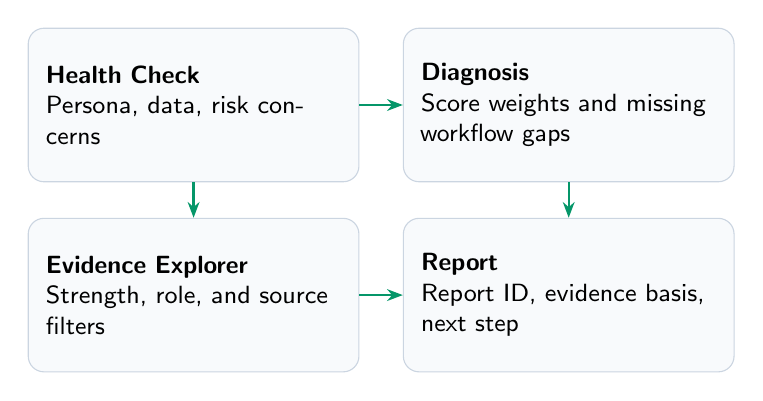
\begin{tikzpicture}[every node/.style={font=\sffamily\small}]
\tikzstyle{screen}=[draw=Border,fill=Light,rounded corners=2mm,minimum width=4.2cm,minimum height=1.95cm,align=left,text width=3.75cm]
\node[screen] (a) {\textbf{Health Check}\\ Persona, data, risk concerns};
\node[screen,right=.55cm of a] (b) {\textbf{Diagnosis}\\ Score weights and missing workflow gaps};
\node[screen,below=.45cm of a] (c) {\textbf{Evidence Explorer}\\ Strength, role, and source filters};
\node[screen,right=.55cm of c] (d) {\textbf{Report}\\ Report ID, evidence basis, next step};
\draw[-{Stealth[length=2mm]},thick,Green] (a)--(b);
\draw[-{Stealth[length=2mm]},thick,Green] (b)--(d);
\draw[-{Stealth[length=2mm]},thick,Green] (a)--(c);
\draw[-{Stealth[length=2mm]},thick,Green] (c)--(d);
\end{tikzpicture}
\caption{Deployed-route montage. The live site exposes a grader path from health-check input to diagnosis, evidence review, and downloadable report.}
\end{figure}

\subsection{Production architecture}

\begin{figure}[H]
\centering
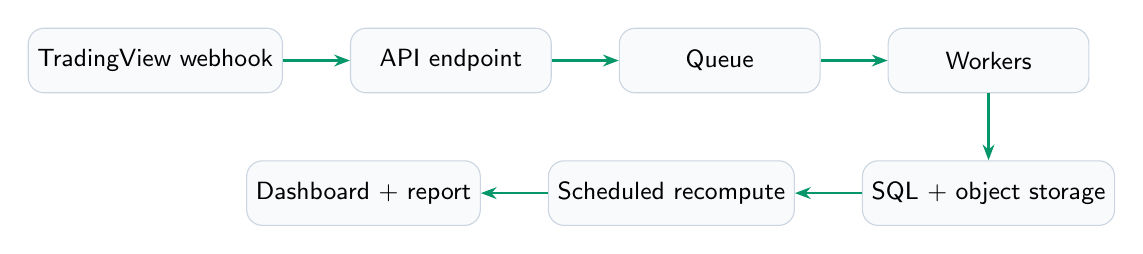
\begin{tikzpicture}[node distance=.85cm, every node/.style={font=\sffamily\small}]
\tikzstyle{box}=[draw=Border,fill=Light,rounded corners=2mm,minimum width=2.55cm,minimum height=.82cm,align=center]
\node[box] (a) {TradingView\ webhook};
\node[box,right=of a] (b) {API\ endpoint};
\node[box,right=of b] (c) {Queue};
\node[box,right=of c] (d) {Workers};
\node[box,below=of d] (e) {SQL + object\ storage};
\node[box,left=of e] (f) {Scheduled\ recompute};
\node[box,left=of f] (g) {Dashboard\ + report};
\draw[-{Stealth[length=2mm]},thick,Green] (a)--(b);
\draw[-{Stealth[length=2mm]},thick,Green] (b)--(c);
\draw[-{Stealth[length=2mm]},thick,Green] (c)--(d);
\draw[-{Stealth[length=2mm]},thick,Green] (d)--(e);
\draw[-{Stealth[length=2mm]},thick,Green] (e)--(f);
\draw[-{Stealth[length=2mm]},thick,Green] (f)--(g);
\end{tikzpicture}
\caption{Production event-driven architecture. The static course artifact implements the delivery and analytics layer; production would add live authorized ingestion and persistent storage.}
\end{figure}

The production version would acknowledge webhooks quickly, enqueue raw payloads, validate idempotency, store raw events and report metadata, recompute reports on a schedule, and expose a dashboard/API/report layer. If privacy-preserving local analytics becomes important, the design can add DuckDB-Wasm or a similar browser-side analytical layer so that heavy report queries run near the user rather than in a central warehouse. At 10x scale, the main additions are a queue, relational metadata store, and daily workers. At 100x scale, the system needs partitioned event tables, object storage retention policy, retry monitoring, and cost-aware pricing for high-frequency users.

\begin{table}[H]
\centering
\caption{Production webhook event contract}
\small
\begin{tabularx}{\textwidth}{>{\raggedright\arraybackslash}p{3.0cm}X}
\toprule
\textbf{Field} & \textbf{Purpose} \\
\midrule
\texttt{event\_id} and \texttt{payload\_hash} & Idempotency and duplicate-event control. \\
\texttt{user\_id}, \texttt{strategy\_id} & User-authorized partitioning and report grouping. \\
\texttt{symbol}, \texttt{timeframe}, \texttt{signal} & Normalized strategy-event metadata. \\
\texttt{alert\_time}, \texttt{alert\_price} & Forward-test attribution anchor. \\
\texttt{payload\_version}, \texttt{raw\_payload\_uri} & Schema evolution and raw audit trail. \\
\bottomrule
\end{tabularx}
\end{table}

\section{Implementation and Reproducibility}

The repository contains all source code, static data, configuration, and documentation needed to run the site locally or through GitHub Pages. The most important implementation files are:

\begin{table}[H]
\centering
\caption{Repository structure}
\scriptsize
\begin{tabularx}{\textwidth}{>{\raggedright\arraybackslash}p{4.8cm}X}
\toprule
\textbf{Path} & \textbf{Role} \\
\midrule
\texttt{docs/index.html} & Static SPA entry point and navigation. \\
\texttt{docs/assets/app.js} & Page rendering and route-specific UI logic. \\
\texttt{docs/assets/scoring.js} & State handling, template recommendation, forward-test attribution, health scoring, and report generation. \\
\texttt{docs/assets/components.js} & Reusable UI helpers, CSV parsing, downloads, and copy actions. \\
\texttt{docs/data/*.csv}, \texttt{*.json} & Static runtime snapshots and public evidence data. \\
\texttt{scripts/validate\_static\_site.py} & Required file and data-key validation. \\
\texttt{scripts/frontend\_smoke\_test.js} & Dependency-free route and data-contract smoke test. \\
\texttt{docs/grader\_guide.md} & Quick path for evaluating the demo. \\
\texttt{docs/data\_lineage.md} & Source-to-report lineage. \\
\texttt{docs/data\_contract.md} & Required fields and runtime assumptions. \\
\texttt{docs/evidence\_governance.md} & Evidence strength labels, interpretation limits, and conservative demand claims. \\
\texttt{docs/public\_evidence\_personas.md} & Synthetic personas derived from public evidence, explicitly not interviews. \\
\texttt{docs/platform...risk\_notes.md} & Platform dependency, privacy, paid-script, and investment-advice boundaries. \\
\bottomrule
\end{tabularx}
\end{table}

The artifact can be run locally with \texttt{python -m http.server 8000 -d docs}. The repository-level validation commands are:

\begin{verbatim}
python scripts/validate_static_site.py
node scripts/frontend_smoke_test.js
\end{verbatim}

\section{Go-to-Market Difficulties and Risk Controls}

The strongest go-to-market risk is trust. Trading-related tools can easily be misunderstood as signal sellers or performance promises. PineGuard mitigates this by positioning itself as workflow validation, not trade recommendation or execution. It also avoids publicly attacking specific paid scripts; reports are user-initiated and based on the user's own observed workflow data. Other major risks are platform dependency, data rights, privacy, cold start, and competition.

\begin{table}[H]
\centering
\caption{Risks and controls}
\small
\begin{tabularx}{\textwidth}{>{\raggedright\arraybackslash}p{3.0cm}X}
\toprule
\textbf{Risk} & \textbf{Control} \\
\midrule
Platform dependency & Use user-authorized alert payloads and user-provided exports; avoid unauthorized scraping. \\
Investment-advice boundary & Do not recommend securities, execute trades, or promise returns. \\
Privacy & Do not collect broker passwords or unnecessary personal data. \\
Cold start & Start with one-time health checks before monthly monitoring. \\
Paid-script disputes & Do not publish accusatory third-party rankings; generate private user-initiated reports from observed data. \\
Competition & Differentiate through evidence-backed reports, alert/outcome history, and audit trails. \\
Unit economics & Price high-frequency users separately because they create disproportionate storage and processing load. \\
\bottomrule
\end{tabularx}
\end{table}

\section{Conclusion}

PineGuard satisfies the assignment goal by connecting technical data processing to a revenue model. The monetized asset is not raw data or alpha. It is auditable workflow validation: a structured product that turns alerts, strategy metadata, market snapshots, and public evidence into a reportable workflow. The current GitHub Pages deployment demonstrates the customer-facing product, while the production architecture explains how the same product would scale with live ingestion, queues, storage, and scheduled processing.

\appendix
\section{References}
{\small
\begin{enumerate}[leftmargin=1.7em,itemsep=.15em,label={[\arabic*]}]
\item TradingView. \emph{Pine Script Documentation: Repainting}. \url{https://www.tradingview.com/pine-script-docs/concepts/repainting/}. Accessed: 19 June 2026.
\item TradingView. \emph{Pine Script Documentation: Strategies}. \url{https://www.tradingview.com/pine-script-docs/concepts/strategies/}. Accessed: 19 June 2026.
\item TradingView. \emph{How to Configure Webhook Alerts}. \url{https://www.tradingview.com/support/solutions/43000529348-how-to-configure-webhook-alerts/}. Accessed: 19 June 2026.
\item TradingView. \emph{Pricing and Plan Features}. \url{https://www.tradingview.com/pricing/}. Accessed: 19 June 2026.
\item Bailey, D. H., Borwein, J., Lopez de Prado, M., and Zhu, Q. J. \emph{The Probability of Backtest Overfitting}. Journal of Computational Finance, 2017.
\item GitHub Docs. \emph{GitHub Pages}. \url{https://docs.github.com/en/pages}. Accessed: 19 June 2026.
\item Apache Kafka Documentation. \emph{Event Streaming Concepts}. \url{https://kafka.apache.org/documentation/}. Accessed: 19 June 2026.
\item Stripe. \emph{Idempotent Requests}. \url{https://docs.stripe.com/api/idempotent_requests}. Accessed: 19 June 2026.
\item DuckDB. \emph{DuckDB-Wasm: Efficient Analytical SQL in the Browser}. \url{https://duckdb.org/2021/10/29/duckdb-wasm}. Accessed: 19 June 2026.
\item TradingView. \emph{Terms of Use, Policies and Disclaimers}. \url{https://www.tradingview.com/policies/}. Accessed: 19 June 2026.
\item TradersPost. \emph{Automated Trading Bot Platform Pricing}. \url{https://traderspost.io/pricing}. Accessed: 19 June 2026.
\item PickMyTrade. \emph{Automated Trading FAQ}. \url{https://pickmytrade.io/general-faq}. Accessed: 19 June 2026.
\item Hootsuite Engineering. \emph{A Scalable, Reliable Webhook Dispatcher Powered by Kafka}. \url{https://medium.com/hootsuite-engineering/a-scalable-reliable-webhook-dispatcher-powered-by-kafka-2dc3d677f16b}. Accessed: 19 June 2026.
\item TradeZella. \emph{Pricing}. \url{https://www.tradezella.com/pricing}. Accessed: 19 June 2026.
\item TradeZella. \emph{TradeZella vs Edgewonk and TraderSync Comparisons}. \url{https://www.tradezella.com/vs/edgewonk}. Accessed: 19 June 2026.
\item TrendSpider. \emph{Trading Platform and Strategy Tools}. \url{https://trendspider.com/}. Accessed: 19 June 2026.
\item QuantConnect. \emph{Pricing}. \url{https://www.quantconnect.com/pricing}. Accessed: 19 June 2026.
\item Stack Overflow. \emph{Pine Script V5: How to Consider Spread and Commission in Backtesting}. \url{https://stackoverflow.com/questions/75297856/pine-script-v5-how-to-consider-the-spread-and-commission-in-backtesting}. Accessed: 19 June 2026.
\item TradingView. \emph{Script Publishing Rules}. \url{https://www.tradingview.com/support/solutions/43000590599-script-publishing-rules/}. Accessed: 19 June 2026.
\item TradingView. \emph{House Rules and Publishing Guide}. \url{https://www.tradingview.com/house-rules/}. Accessed: 19 June 2026.
\end{enumerate}}

\end{document}
